\documentclass[twoside]{book}

% Packages required by doxygen
\usepackage{fixltx2e}
\usepackage{calc}
\usepackage{doxygen}
\usepackage[export]{adjustbox} % also loads graphicx
\usepackage{graphicx}
\usepackage[utf8]{inputenc}
\usepackage{makeidx}
\usepackage{multicol}
\usepackage{multirow}
\PassOptionsToPackage{warn}{textcomp}
\usepackage{textcomp}
\usepackage[nointegrals]{wasysym}
\usepackage[table]{xcolor}

% Font selection
\usepackage[T1]{fontenc}
\usepackage[scaled=.90]{helvet}
\usepackage{courier}
\usepackage{amssymb}
\usepackage{sectsty}
\renewcommand{\familydefault}{\sfdefault}
\allsectionsfont{%
  \fontseries{bc}\selectfont%
  \color{darkgray}%
}
\renewcommand{\DoxyLabelFont}{%
  \fontseries{bc}\selectfont%
  \color{darkgray}%
}
\newcommand{\+}{\discretionary{\mbox{\scriptsize$\hookleftarrow$}}{}{}}

% Page & text layout
\usepackage{geometry}
\geometry{%
  a4paper,%
  top=2.5cm,%
  bottom=2.5cm,%
  left=2.5cm,%
  right=2.5cm%
}
\tolerance=750
\hfuzz=15pt
\hbadness=750
\setlength{\emergencystretch}{15pt}
\setlength{\parindent}{0cm}
\setlength{\parskip}{0.2cm}
\makeatletter
\renewcommand{\paragraph}{%
  \@startsection{paragraph}{4}{0ex}{-1.0ex}{1.0ex}{%
    \normalfont\normalsize\bfseries\SS@parafont%
  }%
}
\renewcommand{\subparagraph}{%
  \@startsection{subparagraph}{5}{0ex}{-1.0ex}{1.0ex}{%
    \normalfont\normalsize\bfseries\SS@subparafont%
  }%
}
\makeatother

% Headers & footers
\usepackage{fancyhdr}
\pagestyle{fancyplain}
\fancyhead[LE]{\fancyplain{}{\bfseries\thepage}}
\fancyhead[CE]{\fancyplain{}{}}
\fancyhead[RE]{\fancyplain{}{\bfseries\leftmark}}
\fancyhead[LO]{\fancyplain{}{\bfseries\rightmark}}
\fancyhead[CO]{\fancyplain{}{}}
\fancyhead[RO]{\fancyplain{}{\bfseries\thepage}}
\fancyfoot[LE]{\fancyplain{}{}}
\fancyfoot[CE]{\fancyplain{}{}}
\fancyfoot[RE]{\fancyplain{}{\bfseries\scriptsize Generated on Thu Nov 19 2015 12\+:37\+:41 for S\+E\+N\+G-\/330-\/\+A2 by Doxygen }}
\fancyfoot[LO]{\fancyplain{}{\bfseries\scriptsize Generated on Thu Nov 19 2015 12\+:37\+:41 for S\+E\+N\+G-\/330-\/\+A2 by Doxygen }}
\fancyfoot[CO]{\fancyplain{}{}}
\fancyfoot[RO]{\fancyplain{}{}}
\renewcommand{\footrulewidth}{0.4pt}
\renewcommand{\chaptermark}[1]{%
  \markboth{#1}{}%
}
\renewcommand{\sectionmark}[1]{%
  \markright{\thesection\ #1}%
}

% Indices & bibliography
\usepackage{natbib}
\usepackage[titles]{tocloft}
\setcounter{tocdepth}{3}
\setcounter{secnumdepth}{5}
\makeindex

% Hyperlinks (required, but should be loaded last)
\usepackage{ifpdf}
\ifpdf
  \usepackage[pdftex,pagebackref=true]{hyperref}
\else
  \usepackage[ps2pdf,pagebackref=true]{hyperref}
\fi
\hypersetup{%
  colorlinks=true,%
  linkcolor=blue,%
  citecolor=blue,%
  unicode%
}

% Custom commands
\newcommand{\clearemptydoublepage}{%
  \newpage{\pagestyle{empty}\cleardoublepage}%
}


%===== C O N T E N T S =====

\begin{document}

% Titlepage & ToC
\hypersetup{pageanchor=false,
             bookmarks=true,
             bookmarksnumbered=true,
             pdfencoding=unicode
            }
\pagenumbering{roman}
\begin{titlepage}
\vspace*{7cm}
\begin{center}%
{\Large S\+E\+N\+G-\/330-\/\+A2 }\\
\vspace*{1cm}
{\large Generated by Doxygen 1.8.10}\\
\vspace*{0.5cm}
{\small Thu Nov 19 2015 12:37:41}\\
\end{center}
\end{titlepage}
\clearemptydoublepage
\tableofcontents
\clearemptydoublepage
\pagenumbering{arabic}
\hypersetup{pageanchor=true}

%--- Begin generated contents ---
\chapter{S\+E\+N\+G-\/330-\/\+A2}
\label{md___users__todd__documents__s_e_n_g-330__a2__s_e_n_g-330-_a2__r_e_a_d_m_e}
\hypertarget{md___users__todd__documents__s_e_n_g-330__a2__s_e_n_g-330-_a2__r_e_a_d_m_e}{}
Text Game

it creats different types of game entity such as rooms, players, and items by different software design pattern. 
\chapter{Hierarchical Index}
\section{Class Hierarchy}
This inheritance list is sorted roughly, but not completely, alphabetically\+:\begin{DoxyCompactList}
\item \contentsline{section}{Entity\+List}{\pageref{class_entity_list}}{}
\item \contentsline{section}{Factory}{\pageref{class_factory}}{}
\item \contentsline{section}{Game\+Entity}{\pageref{class_game_entity}}{}
\begin{DoxyCompactList}
\item \contentsline{section}{Item}{\pageref{class_item}}{}
\item \contentsline{section}{Player}{\pageref{class_player}}{}
\item \contentsline{section}{Room}{\pageref{class_room}}{}
\end{DoxyCompactList}
\end{DoxyCompactList}

\chapter{Class Index}
\section{Class List}
Here are the classes, structs, unions and interfaces with brief descriptions\+:\begin{DoxyCompactList}
\item\contentsline{section}{\hyperlink{class_entity_list}{Entity\+List} }{\pageref{class_entity_list}}{}
\item\contentsline{section}{\hyperlink{class_factory}{Factory} }{\pageref{class_factory}}{}
\item\contentsline{section}{\hyperlink{class_game_entity}{Game\+Entity} }{\pageref{class_game_entity}}{}
\item\contentsline{section}{\hyperlink{class_item}{Item} }{\pageref{class_item}}{}
\item\contentsline{section}{\hyperlink{class_player}{Player} }{\pageref{class_player}}{}
\item\contentsline{section}{\hyperlink{class_room}{Room} }{\pageref{class_room}}{}
\end{DoxyCompactList}

\chapter{File Index}
\section{File List}
Here is a list of all files with brief descriptions\+:\begin{DoxyCompactList}
\item\contentsline{section}{/\+Users/\+Todd/\+Documents/\+S\+E\+N\+G-\/330 A2/\+S\+E\+N\+G-\/330-\/\+A2/\hyperlink{_entity_list_8cpp}{Entity\+List.\+cpp} }{\pageref{_entity_list_8cpp}}{}
\item\contentsline{section}{/\+Users/\+Todd/\+Documents/\+S\+E\+N\+G-\/330 A2/\+S\+E\+N\+G-\/330-\/\+A2/\hyperlink{_entity_list_8h}{Entity\+List.\+h} }{\pageref{_entity_list_8h}}{}
\item\contentsline{section}{/\+Users/\+Todd/\+Documents/\+S\+E\+N\+G-\/330 A2/\+S\+E\+N\+G-\/330-\/\+A2/\hyperlink{_factory_8cpp}{Factory.\+cpp} }{\pageref{_factory_8cpp}}{}
\item\contentsline{section}{/\+Users/\+Todd/\+Documents/\+S\+E\+N\+G-\/330 A2/\+S\+E\+N\+G-\/330-\/\+A2/\hyperlink{_factory_8h}{Factory.\+h} }{\pageref{_factory_8h}}{}
\item\contentsline{section}{/\+Users/\+Todd/\+Documents/\+S\+E\+N\+G-\/330 A2/\+S\+E\+N\+G-\/330-\/\+A2/\hyperlink{_game_entity_8cpp}{Game\+Entity.\+cpp} }{\pageref{_game_entity_8cpp}}{}
\item\contentsline{section}{/\+Users/\+Todd/\+Documents/\+S\+E\+N\+G-\/330 A2/\+S\+E\+N\+G-\/330-\/\+A2/\hyperlink{_game_entity_8h}{Game\+Entity.\+h} }{\pageref{_game_entity_8h}}{}
\item\contentsline{section}{/\+Users/\+Todd/\+Documents/\+S\+E\+N\+G-\/330 A2/\+S\+E\+N\+G-\/330-\/\+A2/\hyperlink{_item_8cpp}{Item.\+cpp} }{\pageref{_item_8cpp}}{}
\item\contentsline{section}{/\+Users/\+Todd/\+Documents/\+S\+E\+N\+G-\/330 A2/\+S\+E\+N\+G-\/330-\/\+A2/\hyperlink{_item_8h}{Item.\+h} }{\pageref{_item_8h}}{}
\item\contentsline{section}{/\+Users/\+Todd/\+Documents/\+S\+E\+N\+G-\/330 A2/\+S\+E\+N\+G-\/330-\/\+A2/\hyperlink{_player_8cpp}{Player.\+cpp} }{\pageref{_player_8cpp}}{}
\item\contentsline{section}{/\+Users/\+Todd/\+Documents/\+S\+E\+N\+G-\/330 A2/\+S\+E\+N\+G-\/330-\/\+A2/\hyperlink{_player_8h}{Player.\+h} }{\pageref{_player_8h}}{}
\item\contentsline{section}{/\+Users/\+Todd/\+Documents/\+S\+E\+N\+G-\/330 A2/\+S\+E\+N\+G-\/330-\/\+A2/\hyperlink{_room_8cpp}{Room.\+cpp} }{\pageref{_room_8cpp}}{}
\item\contentsline{section}{/\+Users/\+Todd/\+Documents/\+S\+E\+N\+G-\/330 A2/\+S\+E\+N\+G-\/330-\/\+A2/\hyperlink{_room_8h}{Room.\+h} }{\pageref{_room_8h}}{}
\end{DoxyCompactList}

\chapter{Class Documentation}
\hypertarget{class_entity_list}{}\section{Entity\+List Class Reference}
\label{class_entity_list}\index{Entity\+List@{Entity\+List}}


{\ttfamily \#include $<$Entity\+List.\+h$>$}

\subsection*{Public Member Functions}
\begin{DoxyCompactItemize}
\item 
\hyperlink{class_entity_list_aed1600f0d729772c4b58f415f724a184}{Entity\+List} ()
\item 
\hyperlink{class_entity_list_a8725ad820c2bfb4fea8557c54d713b9b}{$\sim$\+Entity\+List} ()
\item 
void \hyperlink{class_entity_list_a40295dd300efcf67f02d7d19bdcb1171}{Add\+Entity} (\hyperlink{class_game_entity}{Game\+Entity} $\ast$game\+\_\+entity)
\item 
void \hyperlink{class_entity_list_a413f86f5709a11be52b75fb9c765cc90}{Remove\+Entity} (int id)
\item 
\hyperlink{class_game_entity}{Game\+Entity} $\ast$ \hyperlink{class_entity_list_a91aa2847a1b226bec483bb3c7453f89c}{Get\+Entity} (int id)
\item 
int \hyperlink{class_entity_list_a8f53dae433fa5b9c514a35157ad071b0}{Get\+Entity\+Count} ()
\end{DoxyCompactItemize}


\subsection{Constructor \& Destructor Documentation}
\hypertarget{class_entity_list_aed1600f0d729772c4b58f415f724a184}{}\index{Entity\+List@{Entity\+List}!Entity\+List@{Entity\+List}}
\index{Entity\+List@{Entity\+List}!Entity\+List@{Entity\+List}}
\subsubsection[{Entity\+List()}]{\setlength{\rightskip}{0pt plus 5cm}Entity\+List\+::\+Entity\+List (
\begin{DoxyParamCaption}
{}
\end{DoxyParamCaption}
)}\label{class_entity_list_aed1600f0d729772c4b58f415f724a184}
\hyperlink{_entity_list_8cpp}{Entity\+List.\+cpp} implements the header file \hyperlink{_entity_list_8h}{Entity\+List.\+h} Default constructor that creates an entity list then prints out the information \hypertarget{class_entity_list_a8725ad820c2bfb4fea8557c54d713b9b}{}\index{Entity\+List@{Entity\+List}!````~Entity\+List@{$\sim$\+Entity\+List}}
\index{````~Entity\+List@{$\sim$\+Entity\+List}!Entity\+List@{Entity\+List}}
\subsubsection[{$\sim$\+Entity\+List()}]{\setlength{\rightskip}{0pt plus 5cm}Entity\+List\+::$\sim$\+Entity\+List (
\begin{DoxyParamCaption}
{}
\end{DoxyParamCaption}
)}\label{class_entity_list_a8725ad820c2bfb4fea8557c54d713b9b}
Destructor that delete an entity list then prints out the information 

\subsection{Member Function Documentation}
\hypertarget{class_entity_list_a40295dd300efcf67f02d7d19bdcb1171}{}\index{Entity\+List@{Entity\+List}!Add\+Entity@{Add\+Entity}}
\index{Add\+Entity@{Add\+Entity}!Entity\+List@{Entity\+List}}
\subsubsection[{Add\+Entity(\+Game\+Entity $\ast$game\+\_\+entity)}]{\setlength{\rightskip}{0pt plus 5cm}void Entity\+List\+::\+Add\+Entity (
\begin{DoxyParamCaption}
\item[{{\bf Game\+Entity} $\ast$}]{game\+\_\+entity}
\end{DoxyParamCaption}
)}\label{class_entity_list_a40295dd300efcf67f02d7d19bdcb1171}
Takes the pointer of a game entity and adds the game entity to an existing list. It returns warning if the passed I\+Ds are duplicated. \hypertarget{class_entity_list_a91aa2847a1b226bec483bb3c7453f89c}{}\index{Entity\+List@{Entity\+List}!Get\+Entity@{Get\+Entity}}
\index{Get\+Entity@{Get\+Entity}!Entity\+List@{Entity\+List}}
\subsubsection[{Get\+Entity(int id)}]{\setlength{\rightskip}{0pt plus 5cm}{\bf Game\+Entity} $\ast$ Entity\+List\+::\+Get\+Entity (
\begin{DoxyParamCaption}
\item[{int}]{id}
\end{DoxyParamCaption}
)}\label{class_entity_list_a91aa2847a1b226bec483bb3c7453f89c}
Get the entity corresponding to an I\+D \hypertarget{class_entity_list_a8f53dae433fa5b9c514a35157ad071b0}{}\index{Entity\+List@{Entity\+List}!Get\+Entity\+Count@{Get\+Entity\+Count}}
\index{Get\+Entity\+Count@{Get\+Entity\+Count}!Entity\+List@{Entity\+List}}
\subsubsection[{Get\+Entity\+Count()}]{\setlength{\rightskip}{0pt plus 5cm}int Entity\+List\+::\+Get\+Entity\+Count (
\begin{DoxyParamCaption}
{}
\end{DoxyParamCaption}
)}\label{class_entity_list_a8f53dae433fa5b9c514a35157ad071b0}
Return how many entities are in the list \hypertarget{class_entity_list_a413f86f5709a11be52b75fb9c765cc90}{}\index{Entity\+List@{Entity\+List}!Remove\+Entity@{Remove\+Entity}}
\index{Remove\+Entity@{Remove\+Entity}!Entity\+List@{Entity\+List}}
\subsubsection[{Remove\+Entity(int id)}]{\setlength{\rightskip}{0pt plus 5cm}void Entity\+List\+::\+Remove\+Entity (
\begin{DoxyParamCaption}
\item[{int}]{id}
\end{DoxyParamCaption}
)}\label{class_entity_list_a413f86f5709a11be52b75fb9c765cc90}
Remove an entity corresponding to an I\+D 

The documentation for this class was generated from the following files\+:\begin{DoxyCompactItemize}
\item 
/\+Users/\+Todd/\+Documents/\+S\+E\+N\+G-\/330 A2/\+S\+E\+N\+G-\/330-\/\+A2/\hyperlink{_entity_list_8h}{Entity\+List.\+h}\item 
/\+Users/\+Todd/\+Documents/\+S\+E\+N\+G-\/330 A2/\+S\+E\+N\+G-\/330-\/\+A2/\hyperlink{_entity_list_8cpp}{Entity\+List.\+cpp}\end{DoxyCompactItemize}

\hypertarget{class_factory}{}\section{Factory Class Reference}
\label{class_factory}\index{Factory@{Factory}}


{\ttfamily \#include $<$Factory.\+h$>$}

\subsection*{Static Public Member Functions}
\begin{DoxyCompactItemize}
\item 
static \hyperlink{class_game_entity}{Game\+Entity} $\ast$ \hyperlink{class_factory_a24c5251203420732c7c8cfc496c025ce}{make\+Game\+Entity} (int input)
\end{DoxyCompactItemize}


\subsection{Member Function Documentation}
\hypertarget{class_factory_a24c5251203420732c7c8cfc496c025ce}{}\index{Factory@{Factory}!make\+Game\+Entity@{make\+Game\+Entity}}
\index{make\+Game\+Entity@{make\+Game\+Entity}!Factory@{Factory}}
\subsubsection[{make\+Game\+Entity(int input)}]{\setlength{\rightskip}{0pt plus 5cm}static {\bf Game\+Entity}$\ast$ Factory\+::make\+Game\+Entity (
\begin{DoxyParamCaption}
\item[{int}]{input}
\end{DoxyParamCaption}
)\hspace{0.3cm}{\ttfamily [static]}}\label{class_factory_a24c5251203420732c7c8cfc496c025ce}


The documentation for this class was generated from the following file\+:\begin{DoxyCompactItemize}
\item 
/\+Users/\+Todd/\+Documents/\+S\+E\+N\+G-\/330 A2/\+S\+E\+N\+G-\/330-\/\+A2/\hyperlink{_factory_8h}{Factory.\+h}\end{DoxyCompactItemize}

\hypertarget{class_game_entity}{}\section{Game\+Entity Class Reference}
\label{class_game_entity}\index{Game\+Entity@{Game\+Entity}}


{\ttfamily \#include $<$Game\+Entity.\+h$>$}

Inheritance diagram for Game\+Entity\+:\begin{figure}[H]
\begin{center}
\leavevmode
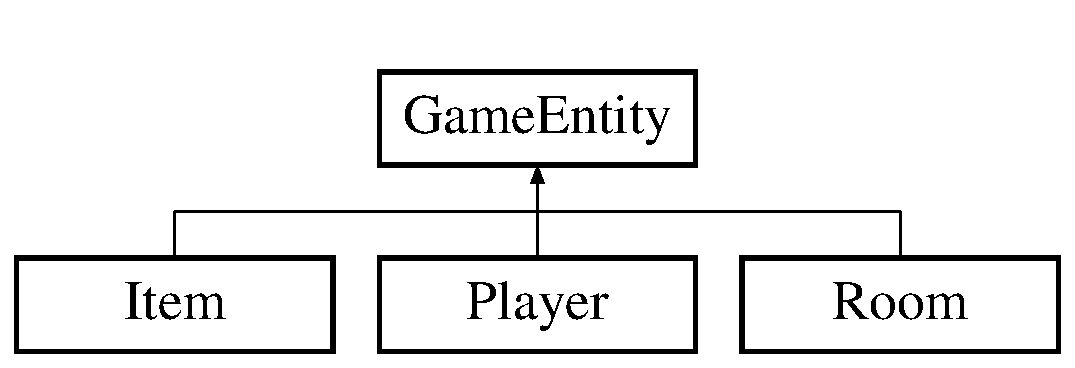
\includegraphics[height=2.000000cm]{class_game_entity}
\end{center}
\end{figure}
\subsection*{Public Member Functions}
\begin{DoxyCompactItemize}
\item 
\hyperlink{class_game_entity_ac534073fe3e7b25d95029c8af622a88e}{Game\+Entity} (int id, std\+::string name)
\item 
\hyperlink{class_game_entity_a941b5c3c653f7526545bd81816e9531a}{Game\+Entity} (int id, std\+::string name, std\+::string description)
\item 
\hyperlink{class_game_entity_a241238b29b5e440107a5b295edf24f9c}{$\sim$\+Game\+Entity} ()
\item 
void \hyperlink{class_game_entity_ac909a518389ee9bc92562b4166340766}{Print} ()
\item 
int \hyperlink{class_game_entity_ad20b660a4f851e9636fdfd15f0d44df0}{Get\+Id} ()
\item 
std\+::string \hyperlink{class_game_entity_ae45ee64de484dec1b16aea85171d9856}{Get\+Name} ()
\item 
std\+::string \hyperlink{class_game_entity_ac8da446a6c6990585b6581fe8537b7bf}{Get\+Description} ()
\item 
void \hyperlink{class_game_entity_a163f5785614921a65aab161491d8c47c}{Set\+Description} (std\+::string description)
\end{DoxyCompactItemize}


\subsection{Detailed Description}
Header file for \hyperlink{class_game_entity}{Game\+Entity} 

\subsection{Constructor \& Destructor Documentation}
\hypertarget{class_game_entity_ac534073fe3e7b25d95029c8af622a88e}{}\index{Game\+Entity@{Game\+Entity}!Game\+Entity@{Game\+Entity}}
\index{Game\+Entity@{Game\+Entity}!Game\+Entity@{Game\+Entity}}
\subsubsection[{Game\+Entity(int id, std\+::string name)}]{\setlength{\rightskip}{0pt plus 5cm}Game\+Entity\+::\+Game\+Entity (
\begin{DoxyParamCaption}
\item[{int}]{id, }
\item[{std\+::string}]{name}
\end{DoxyParamCaption}
)}\label{class_game_entity_ac534073fe3e7b25d95029c8af622a88e}
The public functions have a default constructor, a standard constructor that can set description, a destructor that can remove the entity, and a print function that displays the I\+D, name and description for the entity. Other functions can get the I\+D of the entity, get the name of the entity, and get the description of the entity as well as set a new descroption to the entity.

\hyperlink{_game_entity_8cpp}{Game\+Entity.\+cpp} implements the header file \hyperlink{_game_entity_8h}{Game\+Entity.\+h} Default constructor that creates a game entity by setting a permanent I\+D, name, and a blank description. \hypertarget{class_game_entity_a941b5c3c653f7526545bd81816e9531a}{}\index{Game\+Entity@{Game\+Entity}!Game\+Entity@{Game\+Entity}}
\index{Game\+Entity@{Game\+Entity}!Game\+Entity@{Game\+Entity}}
\subsubsection[{Game\+Entity(int id, std\+::string name, std\+::string description)}]{\setlength{\rightskip}{0pt plus 5cm}Game\+Entity\+::\+Game\+Entity (
\begin{DoxyParamCaption}
\item[{int}]{id, }
\item[{std\+::string}]{name, }
\item[{std\+::string}]{description}
\end{DoxyParamCaption}
)}\label{class_game_entity_a941b5c3c653f7526545bd81816e9531a}
A standard constructor that creates a game entity with a description \hypertarget{class_game_entity_a241238b29b5e440107a5b295edf24f9c}{}\index{Game\+Entity@{Game\+Entity}!````~Game\+Entity@{$\sim$\+Game\+Entity}}
\index{````~Game\+Entity@{$\sim$\+Game\+Entity}!Game\+Entity@{Game\+Entity}}
\subsubsection[{$\sim$\+Game\+Entity()}]{\setlength{\rightskip}{0pt plus 5cm}Game\+Entity\+::$\sim$\+Game\+Entity (
\begin{DoxyParamCaption}
{}
\end{DoxyParamCaption}
)}\label{class_game_entity_a241238b29b5e440107a5b295edf24f9c}
A destructor that removes an entity 

\subsection{Member Function Documentation}
\hypertarget{class_game_entity_ac8da446a6c6990585b6581fe8537b7bf}{}\index{Game\+Entity@{Game\+Entity}!Get\+Description@{Get\+Description}}
\index{Get\+Description@{Get\+Description}!Game\+Entity@{Game\+Entity}}
\subsubsection[{Get\+Description()}]{\setlength{\rightskip}{0pt plus 5cm}std\+::string Game\+Entity\+::\+Get\+Description (
\begin{DoxyParamCaption}
{}
\end{DoxyParamCaption}
)}\label{class_game_entity_ac8da446a6c6990585b6581fe8537b7bf}
Get the description of an entity \hypertarget{class_game_entity_ad20b660a4f851e9636fdfd15f0d44df0}{}\index{Game\+Entity@{Game\+Entity}!Get\+Id@{Get\+Id}}
\index{Get\+Id@{Get\+Id}!Game\+Entity@{Game\+Entity}}
\subsubsection[{Get\+Id()}]{\setlength{\rightskip}{0pt plus 5cm}int Game\+Entity\+::\+Get\+Id (
\begin{DoxyParamCaption}
{}
\end{DoxyParamCaption}
)}\label{class_game_entity_ad20b660a4f851e9636fdfd15f0d44df0}
Get the Id of an entity \hypertarget{class_game_entity_ae45ee64de484dec1b16aea85171d9856}{}\index{Game\+Entity@{Game\+Entity}!Get\+Name@{Get\+Name}}
\index{Get\+Name@{Get\+Name}!Game\+Entity@{Game\+Entity}}
\subsubsection[{Get\+Name()}]{\setlength{\rightskip}{0pt plus 5cm}std\+::string Game\+Entity\+::\+Get\+Name (
\begin{DoxyParamCaption}
{}
\end{DoxyParamCaption}
)}\label{class_game_entity_ae45ee64de484dec1b16aea85171d9856}
Get the name of an entity \hypertarget{class_game_entity_ac909a518389ee9bc92562b4166340766}{}\index{Game\+Entity@{Game\+Entity}!Print@{Print}}
\index{Print@{Print}!Game\+Entity@{Game\+Entity}}
\subsubsection[{Print()}]{\setlength{\rightskip}{0pt plus 5cm}void Game\+Entity\+::\+Print (
\begin{DoxyParamCaption}
{}
\end{DoxyParamCaption}
)}\label{class_game_entity_ac909a518389ee9bc92562b4166340766}
Print the I\+D, name, and description of an entity \hypertarget{class_game_entity_a163f5785614921a65aab161491d8c47c}{}\index{Game\+Entity@{Game\+Entity}!Set\+Description@{Set\+Description}}
\index{Set\+Description@{Set\+Description}!Game\+Entity@{Game\+Entity}}
\subsubsection[{Set\+Description(std\+::string description)}]{\setlength{\rightskip}{0pt plus 5cm}void Game\+Entity\+::\+Set\+Description (
\begin{DoxyParamCaption}
\item[{std\+::string}]{description}
\end{DoxyParamCaption}
)}\label{class_game_entity_a163f5785614921a65aab161491d8c47c}
Change or set the description of an entity 

The documentation for this class was generated from the following files\+:\begin{DoxyCompactItemize}
\item 
/\+Users/\+Todd/\+Documents/\+S\+E\+N\+G-\/330 A2/\+S\+E\+N\+G-\/330-\/\+A2/\hyperlink{_game_entity_8h}{Game\+Entity.\+h}\item 
/\+Users/\+Todd/\+Documents/\+S\+E\+N\+G-\/330 A2/\+S\+E\+N\+G-\/330-\/\+A2/\hyperlink{_game_entity_8cpp}{Game\+Entity.\+cpp}\end{DoxyCompactItemize}

\hypertarget{class_item}{}\section{Item Class Reference}
\label{class_item}\index{Item@{Item}}


{\ttfamily \#include $<$Item.\+h$>$}

Inheritance diagram for Item\+:\begin{figure}[H]
\begin{center}
\leavevmode
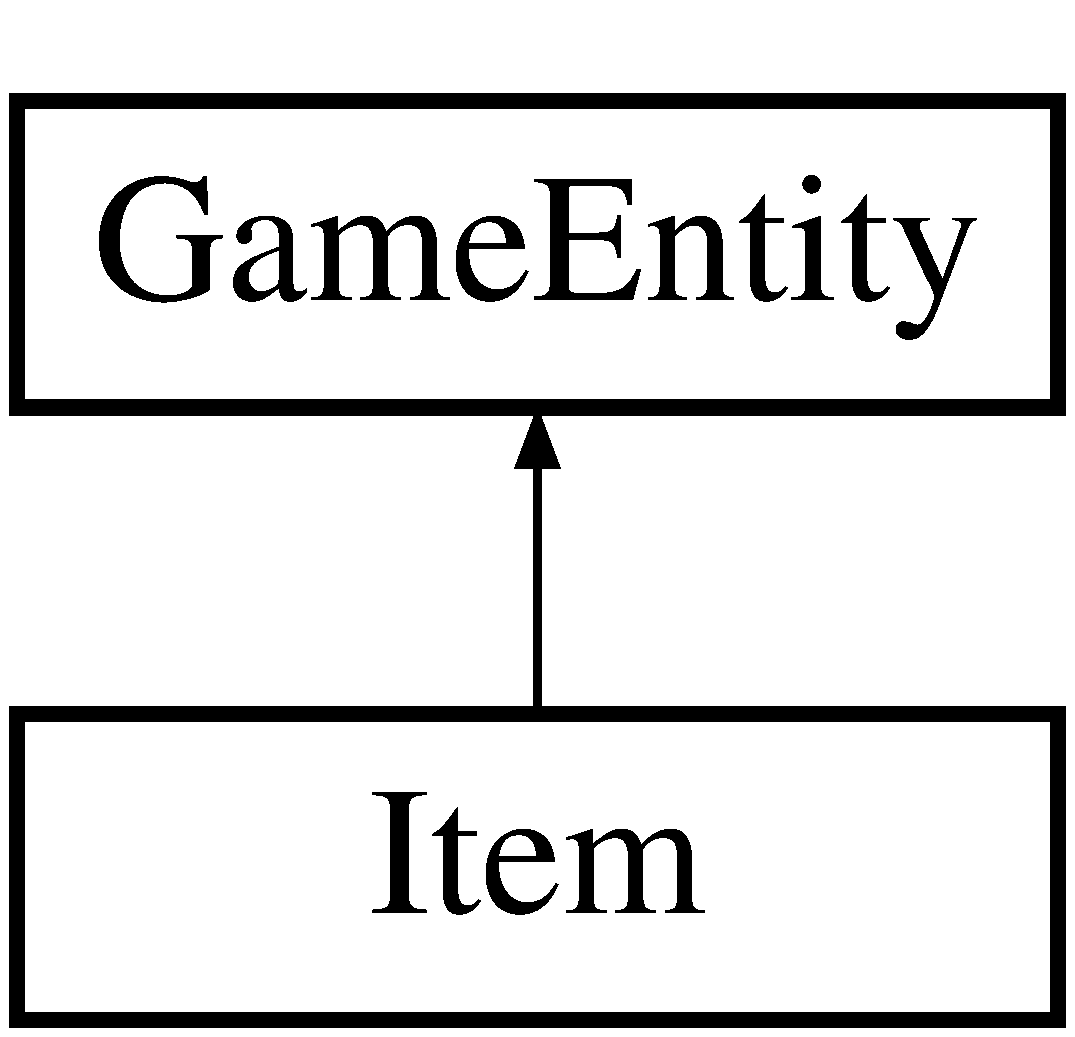
\includegraphics[height=2.000000cm]{class_item}
\end{center}
\end{figure}
\subsection*{Public Member Functions}
\begin{DoxyCompactItemize}
\item 
\hyperlink{class_item_a1de089cb4e92ab58a297c442c69109be}{Item} (int id, std\+::string description)
\item 
\hyperlink{class_item_a7fc39ba8739faa4ea1bd60f1863f770b}{Item} (int id, std\+::string name, std\+::string description)
\item 
\hyperlink{class_item_a11663c84075b78c3ae5e30fdfcd7c458}{$\sim$\+Item} ()
\end{DoxyCompactItemize}


\subsection{Detailed Description}
Header file for item item inherits \hyperlink{class_game_entity}{Game\+Entity} 

\subsection{Constructor \& Destructor Documentation}
\hypertarget{class_item_a1de089cb4e92ab58a297c442c69109be}{}\index{Item@{Item}!Item@{Item}}
\index{Item@{Item}!Item@{Item}}
\subsubsection[{Item(int id, std\+::string description)}]{\setlength{\rightskip}{0pt plus 5cm}Item\+::\+Item (
\begin{DoxyParamCaption}
\item[{int}]{id, }
\item[{std\+::string}]{description}
\end{DoxyParamCaption}
)}\label{class_item_a1de089cb4e92ab58a297c442c69109be}
The public functions contain a default constructor and a standard constructor that takes an I\+D, a name, and a description for the item, and a destructor

\hyperlink{_item_8cpp}{Item.\+cpp} implements the header file \hyperlink{_item_8h}{Item.\+h} Create an item with I\+D and a description \hypertarget{class_item_a7fc39ba8739faa4ea1bd60f1863f770b}{}\index{Item@{Item}!Item@{Item}}
\index{Item@{Item}!Item@{Item}}
\subsubsection[{Item(int id, std\+::string name, std\+::string description)}]{\setlength{\rightskip}{0pt plus 5cm}Item\+::\+Item (
\begin{DoxyParamCaption}
\item[{int}]{id, }
\item[{std\+::string}]{name, }
\item[{std\+::string}]{description}
\end{DoxyParamCaption}
)}\label{class_item_a7fc39ba8739faa4ea1bd60f1863f770b}
Create an item with an I\+D, a name and description \hypertarget{class_item_a11663c84075b78c3ae5e30fdfcd7c458}{}\index{Item@{Item}!````~Item@{$\sim$\+Item}}
\index{````~Item@{$\sim$\+Item}!Item@{Item}}
\subsubsection[{$\sim$\+Item()}]{\setlength{\rightskip}{0pt plus 5cm}Item\+::$\sim$\+Item (
\begin{DoxyParamCaption}
{}
\end{DoxyParamCaption}
)}\label{class_item_a11663c84075b78c3ae5e30fdfcd7c458}
A destructor that destorys an item 

The documentation for this class was generated from the following files\+:\begin{DoxyCompactItemize}
\item 
/\+Users/\+Todd/\+Documents/\+S\+E\+N\+G-\/330 A2/\+S\+E\+N\+G-\/330-\/\+A2/\hyperlink{_item_8h}{Item.\+h}\item 
/\+Users/\+Todd/\+Documents/\+S\+E\+N\+G-\/330 A2/\+S\+E\+N\+G-\/330-\/\+A2/\hyperlink{_item_8cpp}{Item.\+cpp}\end{DoxyCompactItemize}

\hypertarget{class_player}{}\section{Player Class Reference}
\label{class_player}\index{Player@{Player}}


{\ttfamily \#include $<$Player.\+h$>$}

Inheritance diagram for Player\+:\begin{figure}[H]
\begin{center}
\leavevmode
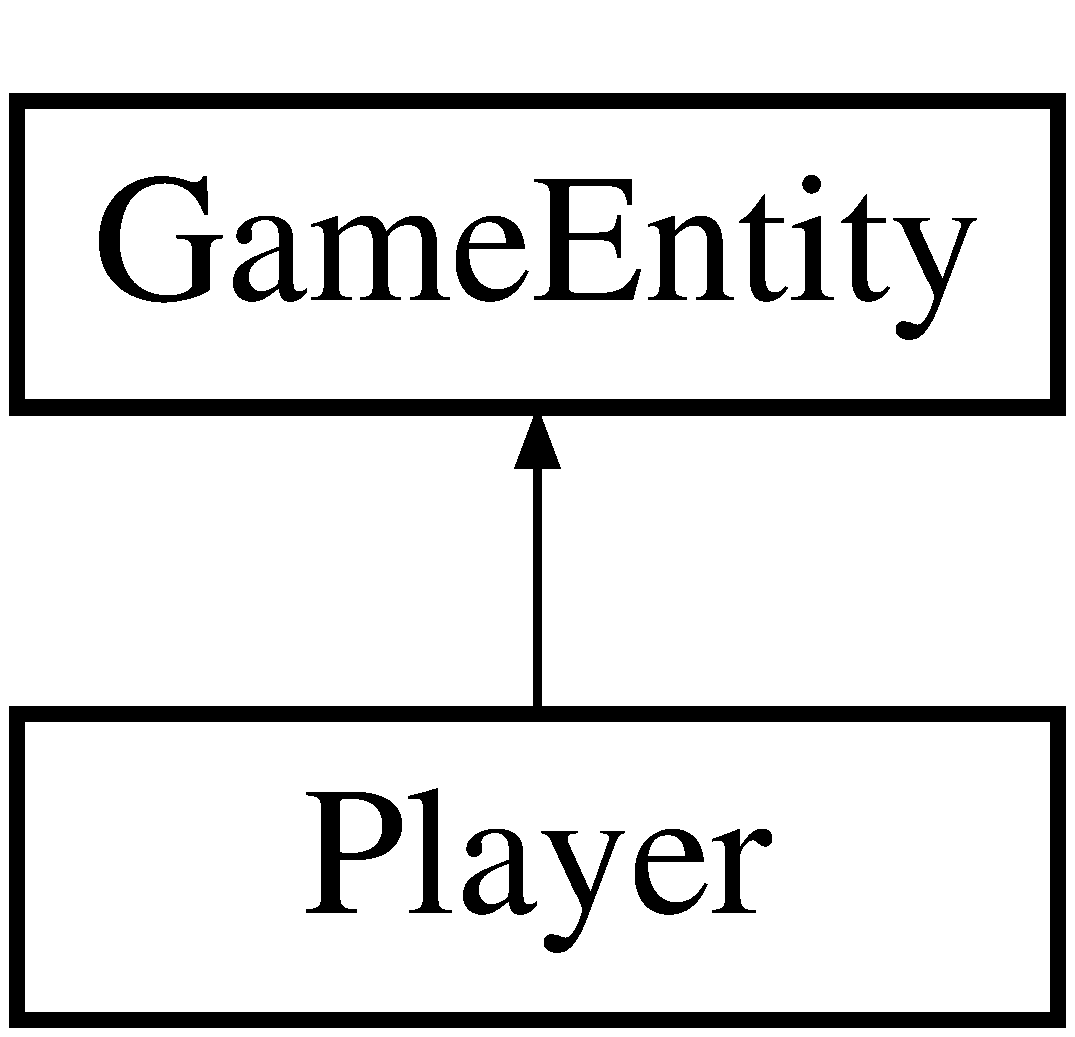
\includegraphics[height=2.000000cm]{class_player}
\end{center}
\end{figure}
\subsection*{Public Member Functions}
\begin{DoxyCompactItemize}
\item 
\hyperlink{class_player_a52b1205956ebebdf8fb8ed36cb96bb38}{Player} (int id, std\+::string name)
\item 
\hyperlink{class_player_a575dc6c353f9db26aa84eafbc7d8470d}{Player} (int id, std\+::string name, int connection\+I\+D\+\_\+)
\item 
\hyperlink{class_player_a749d2c00e1fe0f5c2746f7505a58c062}{$\sim$\+Player} ()
\item 
void \hyperlink{class_player_a3b6ec90fba692a26dd0b7a1152fdd81b}{Print\+Player} ()
\item 
int \hyperlink{class_player_a71946413aa885c5138850a02942a7d34}{Get\+Connection\+I\+D} ()
\end{DoxyCompactItemize}


\subsection{Detailed Description}
The header file of \hyperlink{class_player}{Player} that inherits \hyperlink{class_game_entity}{Game\+Entity} 

\subsection{Constructor \& Destructor Documentation}
\hypertarget{class_player_a52b1205956ebebdf8fb8ed36cb96bb38}{}\index{Player@{Player}!Player@{Player}}
\index{Player@{Player}!Player@{Player}}
\subsubsection[{Player(int id, std\+::string name)}]{\setlength{\rightskip}{0pt plus 5cm}Player\+::\+Player (
\begin{DoxyParamCaption}
\item[{int}]{id, }
\item[{std\+::string}]{name}
\end{DoxyParamCaption}
)}\label{class_player_a52b1205956ebebdf8fb8ed36cb96bb38}
The public functions include a default constructor, a standard constructor, a destructor, and a print function for displaying the information of the player Also Get\+Connection\+I\+D provides the connection id of the player for other classes

\hyperlink{_player_8cpp}{Player.\+cpp} inherits \hyperlink{class_game_entity}{Game\+Entity} implementing the header file \hyperlink{_player_8h}{Player.\+h} A default constructor that creates a player by initial id, a name \hypertarget{class_player_a575dc6c353f9db26aa84eafbc7d8470d}{}\index{Player@{Player}!Player@{Player}}
\index{Player@{Player}!Player@{Player}}
\subsubsection[{Player(int id, std\+::string name, int connection\+I\+D\+\_\+)}]{\setlength{\rightskip}{0pt plus 5cm}Player\+::\+Player (
\begin{DoxyParamCaption}
\item[{int}]{id, }
\item[{std\+::string}]{name, }
\item[{int}]{connection\+I\+D}
\end{DoxyParamCaption}
)}\label{class_player_a575dc6c353f9db26aa84eafbc7d8470d}
A standard constructor that creates a player by initial id, a name, and a connection id \hypertarget{class_player_a749d2c00e1fe0f5c2746f7505a58c062}{}\index{Player@{Player}!````~Player@{$\sim$\+Player}}
\index{````~Player@{$\sim$\+Player}!Player@{Player}}
\subsubsection[{$\sim$\+Player()}]{\setlength{\rightskip}{0pt plus 5cm}Player\+::$\sim$\+Player (
\begin{DoxyParamCaption}
{}
\end{DoxyParamCaption}
)}\label{class_player_a749d2c00e1fe0f5c2746f7505a58c062}
A destructor that removes object player 

\subsection{Member Function Documentation}
\hypertarget{class_player_a71946413aa885c5138850a02942a7d34}{}\index{Player@{Player}!Get\+Connection\+I\+D@{Get\+Connection\+I\+D}}
\index{Get\+Connection\+I\+D@{Get\+Connection\+I\+D}!Player@{Player}}
\subsubsection[{Get\+Connection\+I\+D()}]{\setlength{\rightskip}{0pt plus 5cm}int Player\+::\+Get\+Connection\+I\+D (
\begin{DoxyParamCaption}
{}
\end{DoxyParamCaption}
)}\label{class_player_a71946413aa885c5138850a02942a7d34}
A connection id getter that returns the connection id of the player \hypertarget{class_player_a3b6ec90fba692a26dd0b7a1152fdd81b}{}\index{Player@{Player}!Print\+Player@{Print\+Player}}
\index{Print\+Player@{Print\+Player}!Player@{Player}}
\subsubsection[{Print\+Player()}]{\setlength{\rightskip}{0pt plus 5cm}void Player\+::\+Print\+Player (
\begin{DoxyParamCaption}
{}
\end{DoxyParamCaption}
)}\label{class_player_a3b6ec90fba692a26dd0b7a1152fdd81b}
Print the information of the player 

The documentation for this class was generated from the following files\+:\begin{DoxyCompactItemize}
\item 
/\+Users/\+Todd/\+Documents/\+S\+E\+N\+G-\/330 A2/\+S\+E\+N\+G-\/330-\/\+A2/\hyperlink{_player_8h}{Player.\+h}\item 
/\+Users/\+Todd/\+Documents/\+S\+E\+N\+G-\/330 A2/\+S\+E\+N\+G-\/330-\/\+A2/\hyperlink{_player_8cpp}{Player.\+cpp}\end{DoxyCompactItemize}

\hypertarget{class_room}{}\section{Room Class Reference}
\label{class_room}\index{Room@{Room}}


{\ttfamily \#include $<$Room.\+h$>$}

Inheritance diagram for Room\+:\begin{figure}[H]
\begin{center}
\leavevmode
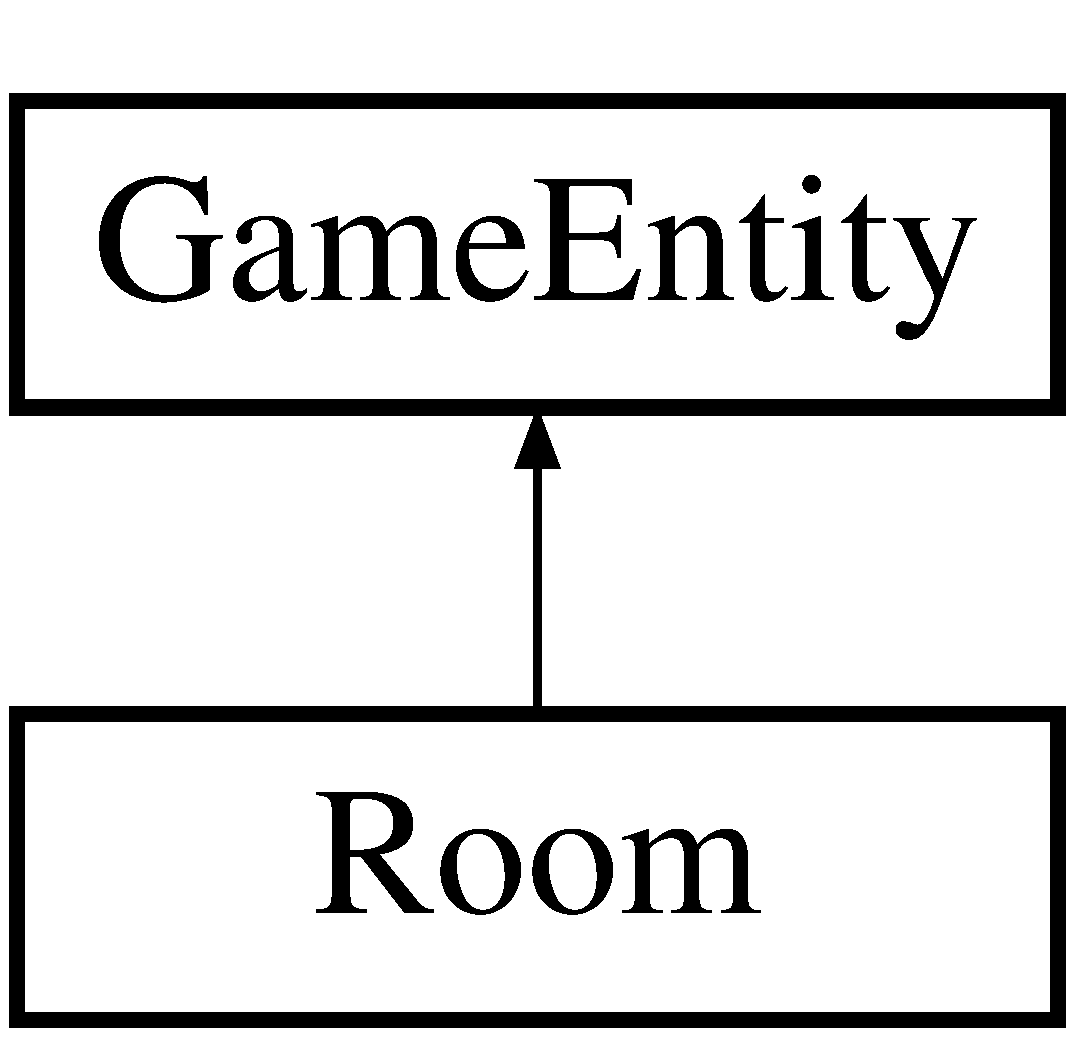
\includegraphics[height=2.000000cm]{class_room}
\end{center}
\end{figure}
\subsection*{Public Member Functions}
\begin{DoxyCompactItemize}
\item 
\hyperlink{class_room_a18d9c7ed056c4bec868cf6939dc90aac}{Room} (int id, std\+::string name)
\item 
\hyperlink{class_room_a2286569deae9af3cafc5716ce72dcbf1}{Room} (int id, std\+::string name, std\+::string description)
\item 
\hyperlink{class_room_a67d5da09983cc53097807fd43ba5481a}{$\sim$\+Room} ()
\item 
void \hyperlink{class_room_a174291564fa1e50053230b844c9dc401}{Add\+Item} (\hyperlink{class_game_entity}{Game\+Entity} $\ast$entity)
\item 
void \hyperlink{class_room_a9d3ded2524dc65d34bcdac48ebfbca4f}{Add\+Exit} (\hyperlink{class_game_entity}{Game\+Entity} $\ast$entity)
\item 
void \hyperlink{class_room_acc80f8dea695a3eee94607fa83531c8c}{Add\+Player} (\hyperlink{class_game_entity}{Game\+Entity} $\ast$entity)
\item 
void \hyperlink{class_room_a2911ca54dcdcde1e2d483d039e01cc62}{Remove\+Item} (int id)
\item 
void \hyperlink{class_room_a18fe6c4958fe671bcb417bc8fa5b2f3a}{Remove\+Exit} (int id)
\item 
void \hyperlink{class_room_a218c9ab86637b3eadf36e51c71299765}{Remove\+Player} (int id)
\item 
\hyperlink{class_game_entity}{Game\+Entity} $\ast$ \hyperlink{class_room_af804da54d2d3649637bd0f9f7a3bf989}{Get\+Exit} (int id)
\item 
\hyperlink{class_game_entity}{Game\+Entity} $\ast$ \hyperlink{class_room_a71f95f978920afe3a2a991d8bcf394f3}{Get\+Item} (int id)
\item 
\hyperlink{class_game_entity}{Game\+Entity} $\ast$ \hyperlink{class_room_a2a3ab0dc562a3bd4ad61ebea0a8ced08}{Get\+Player} (int id)
\end{DoxyCompactItemize}


\subsection{Constructor \& Destructor Documentation}
\hypertarget{class_room_a18d9c7ed056c4bec868cf6939dc90aac}{}\index{Room@{Room}!Room@{Room}}
\index{Room@{Room}!Room@{Room}}
\subsubsection[{Room(int id, std\+::string name)}]{\setlength{\rightskip}{0pt plus 5cm}Room\+::\+Room (
\begin{DoxyParamCaption}
\item[{int}]{id, }
\item[{std\+::string}]{name}
\end{DoxyParamCaption}
)}\label{class_room_a18d9c7ed056c4bec868cf6939dc90aac}
Create a new room with an id and name \hyperlink{class_room}{Room} inherits \hyperlink{class_game_entity}{Game\+Entity} \hypertarget{class_room_a2286569deae9af3cafc5716ce72dcbf1}{}\index{Room@{Room}!Room@{Room}}
\index{Room@{Room}!Room@{Room}}
\subsubsection[{Room(int id, std\+::string name, std\+::string description)}]{\setlength{\rightskip}{0pt plus 5cm}Room\+::\+Room (
\begin{DoxyParamCaption}
\item[{int}]{id, }
\item[{std\+::string}]{name, }
\item[{std\+::string}]{description}
\end{DoxyParamCaption}
)}\label{class_room_a2286569deae9af3cafc5716ce72dcbf1}
Create a new room with an id, name, and description \hypertarget{class_room_a67d5da09983cc53097807fd43ba5481a}{}\index{Room@{Room}!````~Room@{$\sim$\+Room}}
\index{````~Room@{$\sim$\+Room}!Room@{Room}}
\subsubsection[{$\sim$\+Room()}]{\setlength{\rightskip}{0pt plus 5cm}Room\+::$\sim$\+Room (
\begin{DoxyParamCaption}
{}
\end{DoxyParamCaption}
)}\label{class_room_a67d5da09983cc53097807fd43ba5481a}
Remove a room 

\subsection{Member Function Documentation}
\hypertarget{class_room_a9d3ded2524dc65d34bcdac48ebfbca4f}{}\index{Room@{Room}!Add\+Exit@{Add\+Exit}}
\index{Add\+Exit@{Add\+Exit}!Room@{Room}}
\subsubsection[{Add\+Exit(\+Game\+Entity $\ast$entity)}]{\setlength{\rightskip}{0pt plus 5cm}void Room\+::\+Add\+Exit (
\begin{DoxyParamCaption}
\item[{{\bf Game\+Entity} $\ast$}]{roomexit}
\end{DoxyParamCaption}
)}\label{class_room_a9d3ded2524dc65d34bcdac48ebfbca4f}
Each room will have a list of exits (denotes which rooms can be accessed from that room) This function will add an exit to the existing exit list of a room \hypertarget{class_room_a174291564fa1e50053230b844c9dc401}{}\index{Room@{Room}!Add\+Item@{Add\+Item}}
\index{Add\+Item@{Add\+Item}!Room@{Room}}
\subsubsection[{Add\+Item(\+Game\+Entity $\ast$entity)}]{\setlength{\rightskip}{0pt plus 5cm}void Room\+::\+Add\+Item (
\begin{DoxyParamCaption}
\item[{{\bf Game\+Entity} $\ast$}]{item}
\end{DoxyParamCaption}
)}\label{class_room_a174291564fa1e50053230b844c9dc401}
Each room will have a list of items (denotes what items are available to be picked up by characters in the room) This function will add an item to the existing item list of a room \hypertarget{class_room_acc80f8dea695a3eee94607fa83531c8c}{}\index{Room@{Room}!Add\+Player@{Add\+Player}}
\index{Add\+Player@{Add\+Player}!Room@{Room}}
\subsubsection[{Add\+Player(\+Game\+Entity $\ast$entity)}]{\setlength{\rightskip}{0pt plus 5cm}void Room\+::\+Add\+Player (
\begin{DoxyParamCaption}
\item[{{\bf Game\+Entity} $\ast$}]{player}
\end{DoxyParamCaption}
)}\label{class_room_acc80f8dea695a3eee94607fa83531c8c}
Each room will have a list of players (denotes what players are currently in the room at the time) This function will add a player to the existing player list of a room Players get added to the player list when the enter a room \hypertarget{class_room_af804da54d2d3649637bd0f9f7a3bf989}{}\index{Room@{Room}!Get\+Exit@{Get\+Exit}}
\index{Get\+Exit@{Get\+Exit}!Room@{Room}}
\subsubsection[{Get\+Exit(int id)}]{\setlength{\rightskip}{0pt plus 5cm}{\bf Game\+Entity} $\ast$ Room\+::\+Get\+Exit (
\begin{DoxyParamCaption}
\item[{int}]{id}
\end{DoxyParamCaption}
)}\label{class_room_af804da54d2d3649637bd0f9f7a3bf989}
Functions as a check made to see if a certain room exists in a room\textquotesingle{}s exit list (using a room id) Return the \hyperlink{class_game_entity}{Game\+Entity(id)} if it is found in the exit list, else return null if it is not \hypertarget{class_room_a71f95f978920afe3a2a991d8bcf394f3}{}\index{Room@{Room}!Get\+Item@{Get\+Item}}
\index{Get\+Item@{Get\+Item}!Room@{Room}}
\subsubsection[{Get\+Item(int id)}]{\setlength{\rightskip}{0pt plus 5cm}{\bf Game\+Entity} $\ast$ Room\+::\+Get\+Item (
\begin{DoxyParamCaption}
\item[{int}]{id}
\end{DoxyParamCaption}
)}\label{class_room_a71f95f978920afe3a2a991d8bcf394f3}
Gets an item \hyperlink{class_game_entity}{Game\+Entity} using an id if it\textquotesingle{}s in the item list. Return the \hyperlink{class_game_entity}{Game\+Entity(id)} if it is found in the item list, else return null if it is not \hypertarget{class_room_a2a3ab0dc562a3bd4ad61ebea0a8ced08}{}\index{Room@{Room}!Get\+Player@{Get\+Player}}
\index{Get\+Player@{Get\+Player}!Room@{Room}}
\subsubsection[{Get\+Player(int id)}]{\setlength{\rightskip}{0pt plus 5cm}{\bf Game\+Entity} $\ast$ Room\+::\+Get\+Player (
\begin{DoxyParamCaption}
\item[{int}]{id}
\end{DoxyParamCaption}
)}\label{class_room_a2a3ab0dc562a3bd4ad61ebea0a8ced08}
Gets a player \hyperlink{class_game_entity}{Game\+Entity} using an id if it\textquotesingle{}s in the player list. Return the \hyperlink{class_game_entity}{Game\+Entity(id)} if it is found in the player list, else return null if it is not \hypertarget{class_room_a18fe6c4958fe671bcb417bc8fa5b2f3a}{}\index{Room@{Room}!Remove\+Exit@{Remove\+Exit}}
\index{Remove\+Exit@{Remove\+Exit}!Room@{Room}}
\subsubsection[{Remove\+Exit(int id)}]{\setlength{\rightskip}{0pt plus 5cm}void Room\+::\+Remove\+Exit (
\begin{DoxyParamCaption}
\item[{int}]{id}
\end{DoxyParamCaption}
)}\label{class_room_a18fe6c4958fe671bcb417bc8fa5b2f3a}
Remove an exit from the existing exit list of a room \hypertarget{class_room_a2911ca54dcdcde1e2d483d039e01cc62}{}\index{Room@{Room}!Remove\+Item@{Remove\+Item}}
\index{Remove\+Item@{Remove\+Item}!Room@{Room}}
\subsubsection[{Remove\+Item(int id)}]{\setlength{\rightskip}{0pt plus 5cm}void Room\+::\+Remove\+Item (
\begin{DoxyParamCaption}
\item[{int}]{id}
\end{DoxyParamCaption}
)}\label{class_room_a2911ca54dcdcde1e2d483d039e01cc62}
Remove an item from the existing item list of a room Items are removed when a player picks up/takes an item \hypertarget{class_room_a218c9ab86637b3eadf36e51c71299765}{}\index{Room@{Room}!Remove\+Player@{Remove\+Player}}
\index{Remove\+Player@{Remove\+Player}!Room@{Room}}
\subsubsection[{Remove\+Player(int id)}]{\setlength{\rightskip}{0pt plus 5cm}void Room\+::\+Remove\+Player (
\begin{DoxyParamCaption}
\item[{int}]{id}
\end{DoxyParamCaption}
)}\label{class_room_a218c9ab86637b3eadf36e51c71299765}
Remove a player from the existing player list of a room Players are removed when they leave a roome 

The documentation for this class was generated from the following files\+:\begin{DoxyCompactItemize}
\item 
/\+Users/\+Todd/\+Documents/\+S\+E\+N\+G-\/330 A2/\+S\+E\+N\+G-\/330-\/\+A2/\hyperlink{_room_8h}{Room.\+h}\item 
/\+Users/\+Todd/\+Documents/\+S\+E\+N\+G-\/330 A2/\+S\+E\+N\+G-\/330-\/\+A2/\hyperlink{_room_8cpp}{Room.\+cpp}\end{DoxyCompactItemize}

\chapter{File Documentation}
\hypertarget{_entity_list_8cpp}{}\section{/\+Users/\+Todd/\+Documents/\+S\+E\+N\+G-\/330 A2/\+S\+E\+N\+G-\/330-\/\+A2/\+Entity\+List.cpp File Reference}
\label{_entity_list_8cpp}\index{/\+Users/\+Todd/\+Documents/\+S\+E\+N\+G-\/330 A2/\+S\+E\+N\+G-\/330-\/\+A2/\+Entity\+List.\+cpp@{/\+Users/\+Todd/\+Documents/\+S\+E\+N\+G-\/330 A2/\+S\+E\+N\+G-\/330-\/\+A2/\+Entity\+List.\+cpp}}
{\ttfamily \#include \char`\"{}Entity\+List.\+h\char`\"{}}\\*
{\ttfamily \#include $<$iostream$>$}\\*

\hypertarget{_entity_list_8h}{}\section{/\+Users/\+Todd/\+Documents/\+S\+E\+N\+G-\/330 A2/\+S\+E\+N\+G-\/330-\/\+A2/\+Entity\+List.h File Reference}
\label{_entity_list_8h}\index{/\+Users/\+Todd/\+Documents/\+S\+E\+N\+G-\/330 A2/\+S\+E\+N\+G-\/330-\/\+A2/\+Entity\+List.\+h@{/\+Users/\+Todd/\+Documents/\+S\+E\+N\+G-\/330 A2/\+S\+E\+N\+G-\/330-\/\+A2/\+Entity\+List.\+h}}
{\ttfamily \#include \char`\"{}Game\+Entity.\+h\char`\"{}}\\*
{\ttfamily \#include $<$map$>$}\\*
\subsection*{Classes}
\begin{DoxyCompactItemize}
\item 
class \hyperlink{class_entity_list}{Entity\+List}
\end{DoxyCompactItemize}

\hypertarget{_factory_8cpp}{}\section{/\+Users/\+Todd/\+Documents/\+S\+E\+N\+G-\/330 A2/\+S\+E\+N\+G-\/330-\/\+A2/\+Factory.cpp File Reference}
\label{_factory_8cpp}\index{/\+Users/\+Todd/\+Documents/\+S\+E\+N\+G-\/330 A2/\+S\+E\+N\+G-\/330-\/\+A2/\+Factory.\+cpp@{/\+Users/\+Todd/\+Documents/\+S\+E\+N\+G-\/330 A2/\+S\+E\+N\+G-\/330-\/\+A2/\+Factory.\+cpp}}
{\ttfamily \#include \char`\"{}Factory.\+h\char`\"{}}\\*

\hypertarget{_factory_8h}{}\section{/\+Users/\+Todd/\+Documents/\+S\+E\+N\+G-\/330 A2/\+S\+E\+N\+G-\/330-\/\+A2/\+Factory.h File Reference}
\label{_factory_8h}\index{/\+Users/\+Todd/\+Documents/\+S\+E\+N\+G-\/330 A2/\+S\+E\+N\+G-\/330-\/\+A2/\+Factory.\+h@{/\+Users/\+Todd/\+Documents/\+S\+E\+N\+G-\/330 A2/\+S\+E\+N\+G-\/330-\/\+A2/\+Factory.\+h}}
{\ttfamily \#include \char`\"{}Game\+Entity.\+h\char`\"{}}\\*
{\ttfamily \#include \char`\"{}Room.\+h\char`\"{}}\\*
{\ttfamily \#include \char`\"{}Item.\+h\char`\"{}}\\*
{\ttfamily \#include \char`\"{}Player.\+h\char`\"{}}\\*
\subsection*{Classes}
\begin{DoxyCompactItemize}
\item 
class \hyperlink{class_factory}{Factory}
\end{DoxyCompactItemize}

\hypertarget{_game_entity_8cpp}{}\section{/\+Users/\+Todd/\+Documents/\+S\+E\+N\+G-\/330 A2/\+S\+E\+N\+G-\/330-\/\+A2/\+Game\+Entity.cpp File Reference}
\label{_game_entity_8cpp}\index{/\+Users/\+Todd/\+Documents/\+S\+E\+N\+G-\/330 A2/\+S\+E\+N\+G-\/330-\/\+A2/\+Game\+Entity.\+cpp@{/\+Users/\+Todd/\+Documents/\+S\+E\+N\+G-\/330 A2/\+S\+E\+N\+G-\/330-\/\+A2/\+Game\+Entity.\+cpp}}
{\ttfamily \#include \char`\"{}Game\+Entity.\+h\char`\"{}}\\*
{\ttfamily \#include $<$iostream$>$}\\*

\hypertarget{_game_entity_8h}{}\section{/\+Users/\+Todd/\+Documents/\+S\+E\+N\+G-\/330 A2/\+S\+E\+N\+G-\/330-\/\+A2/\+Game\+Entity.h File Reference}
\label{_game_entity_8h}\index{/\+Users/\+Todd/\+Documents/\+S\+E\+N\+G-\/330 A2/\+S\+E\+N\+G-\/330-\/\+A2/\+Game\+Entity.\+h@{/\+Users/\+Todd/\+Documents/\+S\+E\+N\+G-\/330 A2/\+S\+E\+N\+G-\/330-\/\+A2/\+Game\+Entity.\+h}}
{\ttfamily \#include $<$string$>$}\\*
\subsection*{Classes}
\begin{DoxyCompactItemize}
\item 
class \hyperlink{class_game_entity}{Game\+Entity}
\end{DoxyCompactItemize}

\hypertarget{_item_8cpp}{}\section{/\+Users/\+Todd/\+Documents/\+S\+E\+N\+G-\/330 A2/\+S\+E\+N\+G-\/330-\/\+A2/\+Item.cpp File Reference}
\label{_item_8cpp}\index{/\+Users/\+Todd/\+Documents/\+S\+E\+N\+G-\/330 A2/\+S\+E\+N\+G-\/330-\/\+A2/\+Item.\+cpp@{/\+Users/\+Todd/\+Documents/\+S\+E\+N\+G-\/330 A2/\+S\+E\+N\+G-\/330-\/\+A2/\+Item.\+cpp}}
{\ttfamily \#include \char`\"{}Item.\+h\char`\"{}}\\*

\hypertarget{_item_8h}{}\section{/\+Users/\+Todd/\+Documents/\+S\+E\+N\+G-\/330 A2/\+S\+E\+N\+G-\/330-\/\+A2/\+Item.h File Reference}
\label{_item_8h}\index{/\+Users/\+Todd/\+Documents/\+S\+E\+N\+G-\/330 A2/\+S\+E\+N\+G-\/330-\/\+A2/\+Item.\+h@{/\+Users/\+Todd/\+Documents/\+S\+E\+N\+G-\/330 A2/\+S\+E\+N\+G-\/330-\/\+A2/\+Item.\+h}}
{\ttfamily \#include $<$iostream$>$}\\*
{\ttfamily \#include \char`\"{}Game\+Entity.\+h\char`\"{}}\\*
\subsection*{Classes}
\begin{DoxyCompactItemize}
\item 
class \hyperlink{class_item}{Item}
\end{DoxyCompactItemize}

\hypertarget{_player_8cpp}{}\section{/\+Users/\+Todd/\+Documents/\+S\+E\+N\+G-\/330 A2/\+S\+E\+N\+G-\/330-\/\+A2/\+Player.cpp File Reference}
\label{_player_8cpp}\index{/\+Users/\+Todd/\+Documents/\+S\+E\+N\+G-\/330 A2/\+S\+E\+N\+G-\/330-\/\+A2/\+Player.\+cpp@{/\+Users/\+Todd/\+Documents/\+S\+E\+N\+G-\/330 A2/\+S\+E\+N\+G-\/330-\/\+A2/\+Player.\+cpp}}
{\ttfamily \#include \char`\"{}Player.\+h\char`\"{}}\\*

\hypertarget{_player_8h}{}\section{/\+Users/\+Todd/\+Documents/\+S\+E\+N\+G-\/330 A2/\+S\+E\+N\+G-\/330-\/\+A2/\+Player.h File Reference}
\label{_player_8h}\index{/\+Users/\+Todd/\+Documents/\+S\+E\+N\+G-\/330 A2/\+S\+E\+N\+G-\/330-\/\+A2/\+Player.\+h@{/\+Users/\+Todd/\+Documents/\+S\+E\+N\+G-\/330 A2/\+S\+E\+N\+G-\/330-\/\+A2/\+Player.\+h}}
{\ttfamily \#include \char`\"{}Game\+Entity.\+h\char`\"{}}\\*
{\ttfamily \#include $<$iostream$>$}\\*
{\ttfamily \#include $<$string$>$}\\*
\subsection*{Classes}
\begin{DoxyCompactItemize}
\item 
class \hyperlink{class_player}{Player}
\end{DoxyCompactItemize}

\hypertarget{_r_e_a_d_m_e_8md}{}\section{/\+Users/\+Todd/\+Documents/\+S\+E\+N\+G-\/330 A2/\+S\+E\+N\+G-\/330-\/\+A2/\+R\+E\+A\+D\+M\+E.md File Reference}
\label{_r_e_a_d_m_e_8md}\index{/\+Users/\+Todd/\+Documents/\+S\+E\+N\+G-\/330 A2/\+S\+E\+N\+G-\/330-\/\+A2/\+R\+E\+A\+D\+M\+E.\+md@{/\+Users/\+Todd/\+Documents/\+S\+E\+N\+G-\/330 A2/\+S\+E\+N\+G-\/330-\/\+A2/\+R\+E\+A\+D\+M\+E.\+md}}

\hypertarget{_room_8cpp}{}\section{/\+Users/\+Todd/\+Documents/\+S\+E\+N\+G-\/330 A2/\+S\+E\+N\+G-\/330-\/\+A2/\+Room.cpp File Reference}
\label{_room_8cpp}\index{/\+Users/\+Todd/\+Documents/\+S\+E\+N\+G-\/330 A2/\+S\+E\+N\+G-\/330-\/\+A2/\+Room.\+cpp@{/\+Users/\+Todd/\+Documents/\+S\+E\+N\+G-\/330 A2/\+S\+E\+N\+G-\/330-\/\+A2/\+Room.\+cpp}}
{\ttfamily \#include \char`\"{}Room.\+h\char`\"{}}\\*

\hypertarget{_room_8h}{}\section{/\+Users/\+Todd/\+Documents/\+S\+E\+N\+G-\/330 A2/\+S\+E\+N\+G-\/330-\/\+A2/\+Room.h File Reference}
\label{_room_8h}\index{/\+Users/\+Todd/\+Documents/\+S\+E\+N\+G-\/330 A2/\+S\+E\+N\+G-\/330-\/\+A2/\+Room.\+h@{/\+Users/\+Todd/\+Documents/\+S\+E\+N\+G-\/330 A2/\+S\+E\+N\+G-\/330-\/\+A2/\+Room.\+h}}
{\ttfamily \#include $<$iostream$>$}\\*
{\ttfamily \#include \char`\"{}Entity\+List.\+h\char`\"{}}\\*
{\ttfamily \#include \char`\"{}Game\+Entity.\+h\char`\"{}}\\*
\subsection*{Classes}
\begin{DoxyCompactItemize}
\item 
class \hyperlink{class_room}{Room}
\end{DoxyCompactItemize}

%--- End generated contents ---

% Index
\backmatter
\newpage
\phantomsection
\clearemptydoublepage
\addcontentsline{toc}{chapter}{Index}
\printindex

\end{document}
